\documentclass[]{article}
\usepackage{lmodern}
\usepackage{amssymb,amsmath}
\usepackage{ifxetex,ifluatex}
\usepackage{fixltx2e} % provides \textsubscript
\ifnum 0\ifxetex 1\fi\ifluatex 1\fi=0 % if pdftex
  \usepackage[T1]{fontenc}
  \usepackage[utf8]{inputenc}
\else % if luatex or xelatex
  \ifxetex
    \usepackage{mathspec}
    \usepackage{xltxtra,xunicode}
  \else
    \usepackage{fontspec}
  \fi
  \defaultfontfeatures{Mapping=tex-text,Scale=MatchLowercase}
  \newcommand{\euro}{€}
\fi
% use upquote if available, for straight quotes in verbatim environments
\IfFileExists{upquote.sty}{\usepackage{upquote}}{}
% use microtype if available
\IfFileExists{microtype.sty}{%
\usepackage{microtype}
\UseMicrotypeSet[protrusion]{basicmath} % disable protrusion for tt fonts
}{}
\usepackage[margin=1in]{geometry}
\usepackage{color}
\usepackage{fancyvrb}
\newcommand{\VerbBar}{|}
\newcommand{\VERB}{\Verb[commandchars=\\\{\}]}
\DefineVerbatimEnvironment{Highlighting}{Verbatim}{commandchars=\\\{\}}
% Add ',fontsize=\small' for more characters per line
\usepackage{framed}
\definecolor{shadecolor}{RGB}{248,248,248}
\newenvironment{Shaded}{\begin{snugshade}}{\end{snugshade}}
\newcommand{\KeywordTok}[1]{\textcolor[rgb]{0.13,0.29,0.53}{\textbf{{#1}}}}
\newcommand{\DataTypeTok}[1]{\textcolor[rgb]{0.13,0.29,0.53}{{#1}}}
\newcommand{\DecValTok}[1]{\textcolor[rgb]{0.00,0.00,0.81}{{#1}}}
\newcommand{\BaseNTok}[1]{\textcolor[rgb]{0.00,0.00,0.81}{{#1}}}
\newcommand{\FloatTok}[1]{\textcolor[rgb]{0.00,0.00,0.81}{{#1}}}
\newcommand{\CharTok}[1]{\textcolor[rgb]{0.31,0.60,0.02}{{#1}}}
\newcommand{\StringTok}[1]{\textcolor[rgb]{0.31,0.60,0.02}{{#1}}}
\newcommand{\CommentTok}[1]{\textcolor[rgb]{0.56,0.35,0.01}{\textit{{#1}}}}
\newcommand{\OtherTok}[1]{\textcolor[rgb]{0.56,0.35,0.01}{{#1}}}
\newcommand{\AlertTok}[1]{\textcolor[rgb]{0.94,0.16,0.16}{{#1}}}
\newcommand{\FunctionTok}[1]{\textcolor[rgb]{0.00,0.00,0.00}{{#1}}}
\newcommand{\RegionMarkerTok}[1]{{#1}}
\newcommand{\ErrorTok}[1]{\textbf{{#1}}}
\newcommand{\NormalTok}[1]{{#1}}
\usepackage{graphicx}
\makeatletter
\def\maxwidth{\ifdim\Gin@nat@width>\linewidth\linewidth\else\Gin@nat@width\fi}
\def\maxheight{\ifdim\Gin@nat@height>\textheight\textheight\else\Gin@nat@height\fi}
\makeatother
% Scale images if necessary, so that they will not overflow the page
% margins by default, and it is still possible to overwrite the defaults
% using explicit options in \includegraphics[width, height, ...]{}
\setkeys{Gin}{width=\maxwidth,height=\maxheight,keepaspectratio}
\ifxetex
  \usepackage[setpagesize=false, % page size defined by xetex
              unicode=false, % unicode breaks when used with xetex
              xetex]{hyperref}
\else
  \usepackage[unicode=true]{hyperref}
\fi
\hypersetup{breaklinks=true,
            bookmarks=true,
            pdfauthor={},
            pdftitle={},
            colorlinks=true,
            citecolor=blue,
            urlcolor=blue,
            linkcolor=magenta,
            pdfborder={0 0 0}}
\urlstyle{same}  % don't use monospace font for urls
\setlength{\parindent}{0pt}
\setlength{\parskip}{6pt plus 2pt minus 1pt}
\setlength{\emergencystretch}{3em}  % prevent overfull lines
\setcounter{secnumdepth}{0}

%%% Use protect on footnotes to avoid problems with footnotes in titles
\let\rmarkdownfootnote\footnote%
\def\footnote{\protect\rmarkdownfootnote}

%%% Change title format to be more compact
\usepackage{titling}

% Create subtitle command for use in maketitle
\newcommand{\subtitle}[1]{
  \posttitle{
    \begin{center}\large#1\end{center}
    }
}

\setlength{\droptitle}{-2em}
  \title{}
  \pretitle{\vspace{\droptitle}}
  \posttitle{}
  \author{}
  \preauthor{}\postauthor{}
  \date{}
  \predate{}\postdate{}



\begin{document}

\maketitle


\section{Regression Models}\label{regression-models}

\subsubsection{Peer Assessment 1:
PA1\_template}\label{peer-assessment-1-pa1ux5ftemplate}

\subsubsection{Introduction}\label{introduction}

This document presents the results of Peer Assessment 1 for the Coursera
course: Regression Models. This assessment required analysis on a data
set of a collection of cars. In particular, exploring the relationship
between a set of variables and miles per gallon.

\subsubsection{Data}\label{data}

This assignment makes use of the `mtcars' data set. The data was
extracted from the 1974 Motor Trend US magazine, and comprises fuel
consumption and 10 aspects of automobile design and performance for 32
automobiles (1973-74 models).

\begin{itemize}
\itemsep1pt\parskip0pt\parsep0pt
\item
  Dataset:
  \href{https://stat.ethz.ch/R-manual/R-devel/library/datasets/html/mtcars.html}{mtcars
  data}
\end{itemize}

It consists of 32 observations on 11 variables:

\begin{itemize}
\itemsep1pt\parskip0pt\parsep0pt
\item
  \texttt{mpg}: Miles per US gallon
\item
  \texttt{cyl}: Number of cylinders
\item
  \texttt{disp}: Displacement (cubic inches)
\item
  \texttt{hp}: Gross horsepower
\item
  \texttt{drat}: Rear axle ratio
\item
  \texttt{wt}: Weight (lb / 1000)
\item
  \texttt{qsec}: 1 / 4 mile time
\item
  \texttt{vs}: V/S
\item
  \texttt{am}: Transmission (0 = automatic, 1 = manual)
\item
  \texttt{gear}: Number of forward gears
\item
  \texttt{carb}: Number of carburetors
\end{itemize}

\subsubsection{1. Loading Data/Packages}\label{loading-datapackages}

\begin{Shaded}
\begin{Highlighting}[]
\NormalTok{for (package in }\KeywordTok{c}\NormalTok{(}\StringTok{'ggplot2'}\NormalTok{, }\StringTok{'stats'}\NormalTok{, }\StringTok{'graphics'}\NormalTok{, }\StringTok{'GGally'}\NormalTok{, }\StringTok{'caret'}\NormalTok{, }\StringTok{'reshape2'}\NormalTok{)) \{}
  
    \NormalTok{if (!}\KeywordTok{require}\NormalTok{(package, }\DataTypeTok{character.only =} \OtherTok{TRUE}\NormalTok{, }\DataTypeTok{quietly =} \OtherTok{FALSE}\NormalTok{)) \{}
        \KeywordTok{install.packages}\NormalTok{(package)}
        \KeywordTok{library}\NormalTok{(package, }\DataTypeTok{character.only =} \OtherTok{TRUE}\NormalTok{)}
    \NormalTok{\}}
\NormalTok{\}}

\KeywordTok{data}\NormalTok{(mtcars)}
\NormalTok{data_mtcars <-}\StringTok{ }\NormalTok{mtcars}
\end{Highlighting}
\end{Shaded}

\subsubsection{2. Subset and Plot Relevant
Data:}\label{subset-and-plot-relevant-data}

\begin{Shaded}
\begin{Highlighting}[]
\NormalTok{data_mpgtrans <-}\StringTok{ }\KeywordTok{data.frame}\NormalTok{(}
  \DataTypeTok{mpg =} \NormalTok{data_mtcars[, }\DecValTok{1}\NormalTok{],}
  \DataTypeTok{cyl =} \NormalTok{data_mtcars[, }\DecValTok{2}\NormalTok{],}
  \DataTypeTok{disp =} \NormalTok{data_mtcars[, }\DecValTok{3}\NormalTok{],}
  \DataTypeTok{hp =} \NormalTok{data_mtcars[, }\DecValTok{4}\NormalTok{],}
  \DataTypeTok{drat =} \NormalTok{data_mtcars[, }\DecValTok{5}\NormalTok{],}
  \DataTypeTok{wt =} \NormalTok{data_mtcars[, }\DecValTok{6}\NormalTok{],}
  \DataTypeTok{qsec =} \NormalTok{data_mtcars[, }\DecValTok{7}\NormalTok{],}
  \DataTypeTok{vs =} \NormalTok{data_mtcars[, }\DecValTok{8}\NormalTok{],}
  \DataTypeTok{am =} \KeywordTok{factor}\NormalTok{(data_mtcars[, }\DecValTok{9}\NormalTok{], }\DataTypeTok{labels =} \KeywordTok{c}\NormalTok{(}\StringTok{"Automatic"}\NormalTok{, }\StringTok{"Manual"}\NormalTok{)),}
  \DataTypeTok{gear =} \NormalTok{data_mtcars[, }\DecValTok{10}\NormalTok{],}
  \DataTypeTok{carb =} \NormalTok{data_mtcars[, }\DecValTok{11}\NormalTok{])}
\end{Highlighting}
\end{Shaded}

\subsubsection{3. Exploratory Data
Analysis:}\label{exploratory-data-analysis}

The appendix contains figures used for basic exploratory data analysis.

Figure 1 shows pair relationships between each variable categorised by
`am'. At a high level, the pair relationships suggest correlation
between many of the dataset variables. `mpg' in particular seems to have
a strong correlation with variables `cyl', `disp', `hp' and `wt'. Figure
2 shows a histogram of `mpg' also categorised by `am'. No outliers are
identified, however the distribution does seem to exhibit a slight
positive skew. Finally, figure 3 shows a boxplot between `mpg' and `am'.
This figure suggests manual cars achieve greater mpg than automatic
cars.

\subsubsection{4. Statistical Inference:}\label{statistical-inference}

\paragraph{Test null hypothesis that there is no difference between
automatic and manual cars in terms of
mpg:}\label{test-null-hypothesis-that-there-is-no-difference-between-automatic-and-manual-cars-in-terms-of-mpg}

\begin{verbatim}
## 
##  Welch Two Sample t-test
## 
## data:  data_mpgtrans.at and data_mpgtrans.mt
## t = -3.7671, df = 18.332, p-value = 0.001374
## alternative hypothesis: true difference in means is not equal to 0
## 95 percent confidence interval:
##  -11.280194  -3.209684
## sample estimates:
## mean of x mean of y 
##  17.14737  24.39231
\end{verbatim}

Based on the reported p-value and using 0.05 as the criteria, the null
hypothesis should be rejected. This suggests a statistical significant
difference between automatic car and manual car in terms of achieved
mpg.

\subsubsection{5. Model Selection:}\label{model-selection}

\paragraph{Create models with various selection method and
criteria:}\label{create-models-with-various-selection-method-and-criteria}

Several linear regression models are built, each using `mpg' as the
dependent variable.

\paragraph{Model 1: Linear model to explain mpg as a function of
transmission
type.}\label{model-1-linear-model-to-explain-mpg-as-a-function-of-transmission-type.}

\begin{verbatim}
## 
## Call:
## lm(formula = .outcome ~ ., data = dat)
## 
## Residuals:
##     Min      1Q  Median      3Q     Max 
## -9.3923 -3.0923 -0.2974  3.2439  9.5077 
## 
## Coefficients:
##             Estimate Std. Error t value Pr(>|t|)    
## (Intercept)   17.147      1.125  15.247 1.13e-15 ***
## am             7.245      1.764   4.106 0.000285 ***
## ---
## Signif. codes:  0 '***' 0.001 '**' 0.01 '*' 0.05 '.' 0.1 ' ' 1
## 
## Residual standard error: 4.902 on 30 degrees of freedom
## Multiple R-squared:  0.3598, Adjusted R-squared:  0.3385 
## F-statistic: 16.86 on 1 and 30 DF,  p-value: 0.000285
\end{verbatim}

Model shows significant coefficient for `am' explanatory variable (p
\textless{}= 0.05), however model has a low R-square value.

\paragraph{Model 2: Searched linear model using lmStepAIC method,
backward
direction.}\label{model-2-searched-linear-model-using-lmstepaic-method-backward-direction.}

\begin{verbatim}
## 
## Call:
## lm(formula = .outcome ~ wt + qsec + am, data = dat)
## 
## Residuals:
##     Min      1Q  Median      3Q     Max 
## -3.4811 -1.5555 -0.7257  1.4110  4.6610 
## 
## Coefficients:
##             Estimate Std. Error t value Pr(>|t|)    
## (Intercept)   9.6178     6.9596   1.382 0.177915    
## wt           -3.9165     0.7112  -5.507 6.95e-06 ***
## qsec          1.2259     0.2887   4.247 0.000216 ***
## am            2.9358     1.4109   2.081 0.046716 *  
## ---
## Signif. codes:  0 '***' 0.001 '**' 0.01 '*' 0.05 '.' 0.1 ' ' 1
## 
## Residual standard error: 2.459 on 28 degrees of freedom
## Multiple R-squared:  0.8497, Adjusted R-squared:  0.8336 
## F-statistic: 52.75 on 3 and 28 DF,  p-value: 1.21e-11
\end{verbatim}

Model shows significant coefficient for all included explanatory
variables (p \textless{}= 0.05), 83\% adjusted R-squared value.

\paragraph{Model 3: Searched linear model using lmStepAIC method,
forward
direction.}\label{model-3-searched-linear-model-using-lmstepaic-method-forward-direction.}

\begin{verbatim}
## 
## Call:
## lm(formula = .outcome ~ cyl + disp + hp + drat + wt + qsec + 
##     vs + am + gear + carb, data = dat)
## 
## Residuals:
##     Min      1Q  Median      3Q     Max 
## -3.4506 -1.6044 -0.1196  1.2193  4.6271 
## 
## Coefficients:
##             Estimate Std. Error t value Pr(>|t|)  
## (Intercept) 12.30337   18.71788   0.657   0.5181  
## cyl         -0.11144    1.04502  -0.107   0.9161  
## disp         0.01334    0.01786   0.747   0.4635  
## hp          -0.02148    0.02177  -0.987   0.3350  
## drat         0.78711    1.63537   0.481   0.6353  
## wt          -3.71530    1.89441  -1.961   0.0633 .
## qsec         0.82104    0.73084   1.123   0.2739  
## vs           0.31776    2.10451   0.151   0.8814  
## am           2.52023    2.05665   1.225   0.2340  
## gear         0.65541    1.49326   0.439   0.6652  
## carb        -0.19942    0.82875  -0.241   0.8122  
## ---
## Signif. codes:  0 '***' 0.001 '**' 0.01 '*' 0.05 '.' 0.1 ' ' 1
## 
## Residual standard error: 2.65 on 21 degrees of freedom
## Multiple R-squared:  0.869,  Adjusted R-squared:  0.8066 
## F-statistic: 13.93 on 10 and 21 DF,  p-value: 3.793e-07
\end{verbatim}

Model shows insignificant coefficient for all included explanatory
variables (p \textless{}= 0.05), 80\% adjusted R-squared value.

\paragraph{Select optimal model:}\label{select-optimal-model}

Of the three tested models, model 2 is selected as it has the highest
adjusted R-squared value with significant explanatory variables (p
\textless{}= 0.05).

\subsubsection{6. Regression Analysis:}\label{regression-analysis}

The coefficients for the selected model suggest that (when holding all
other explanatory variables constant), an increase in `wt' results in a
decrease in `mpg', an increase in `qsec' results in an increase in
`mpg', and finally, cars with manual transmissions (`am' = 1) provide an
increase in `mpg'.

Figure 4 suggest that the selected model provides a good fit to actual
`mpg' data. Figure 5 shows fitted residuals which are randomly scattered
with no particular pattern.

\subsubsection{7. Conclusion:}\label{conclusion}

The selected model suggests that a cars weight, quarter-mile time and
transmission type are reasonable explanatory variables to use in
determining its mile per gallon performance. Cars with a greater weight,
lower (quicker) quarter mile time and automatic transmissions achieve
less miles per gallon, while cars with less weight, higher (slower)
quarter mile times and manual transmission achieve greater miles per
gallon.

\subsubsection{8. Appendix:}\label{appendix}

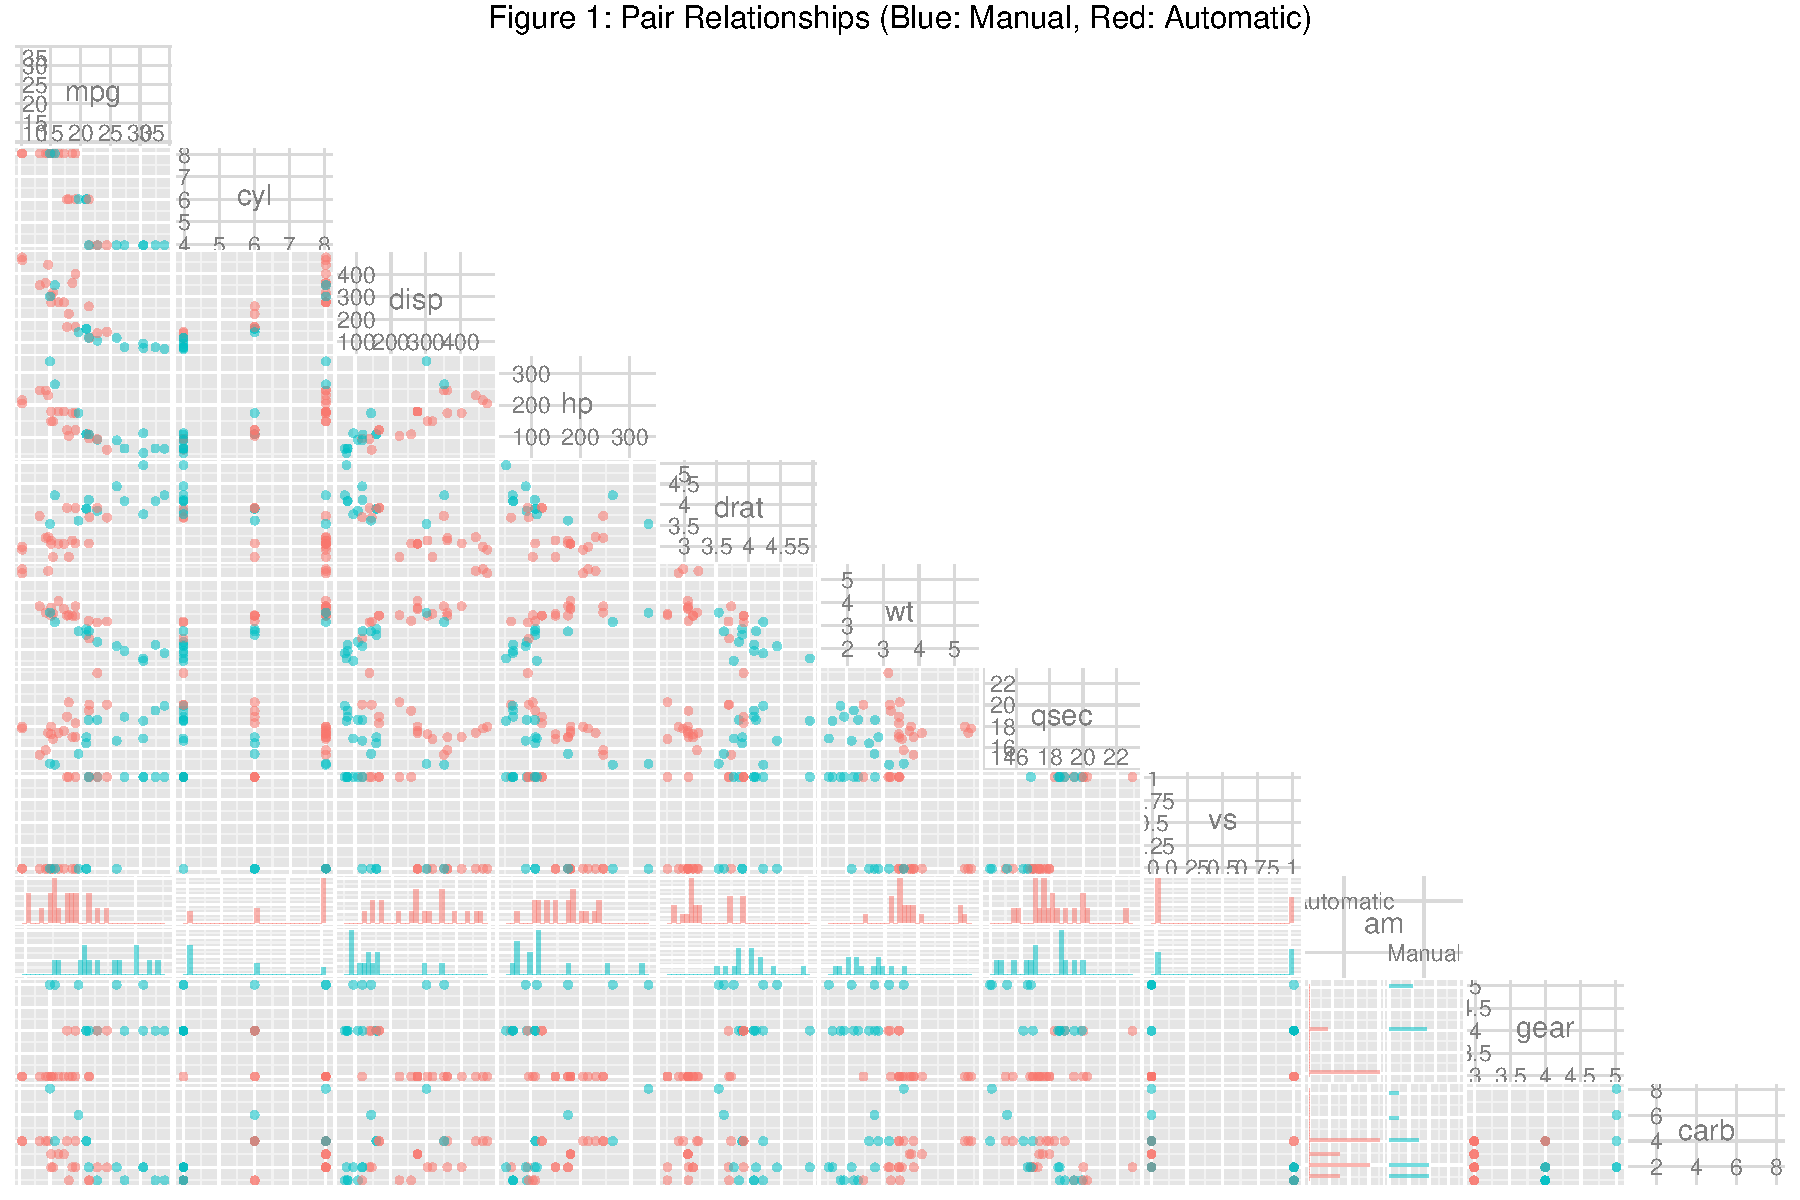
\includegraphics{figure/unnamed-chunk-10-1.pdf}

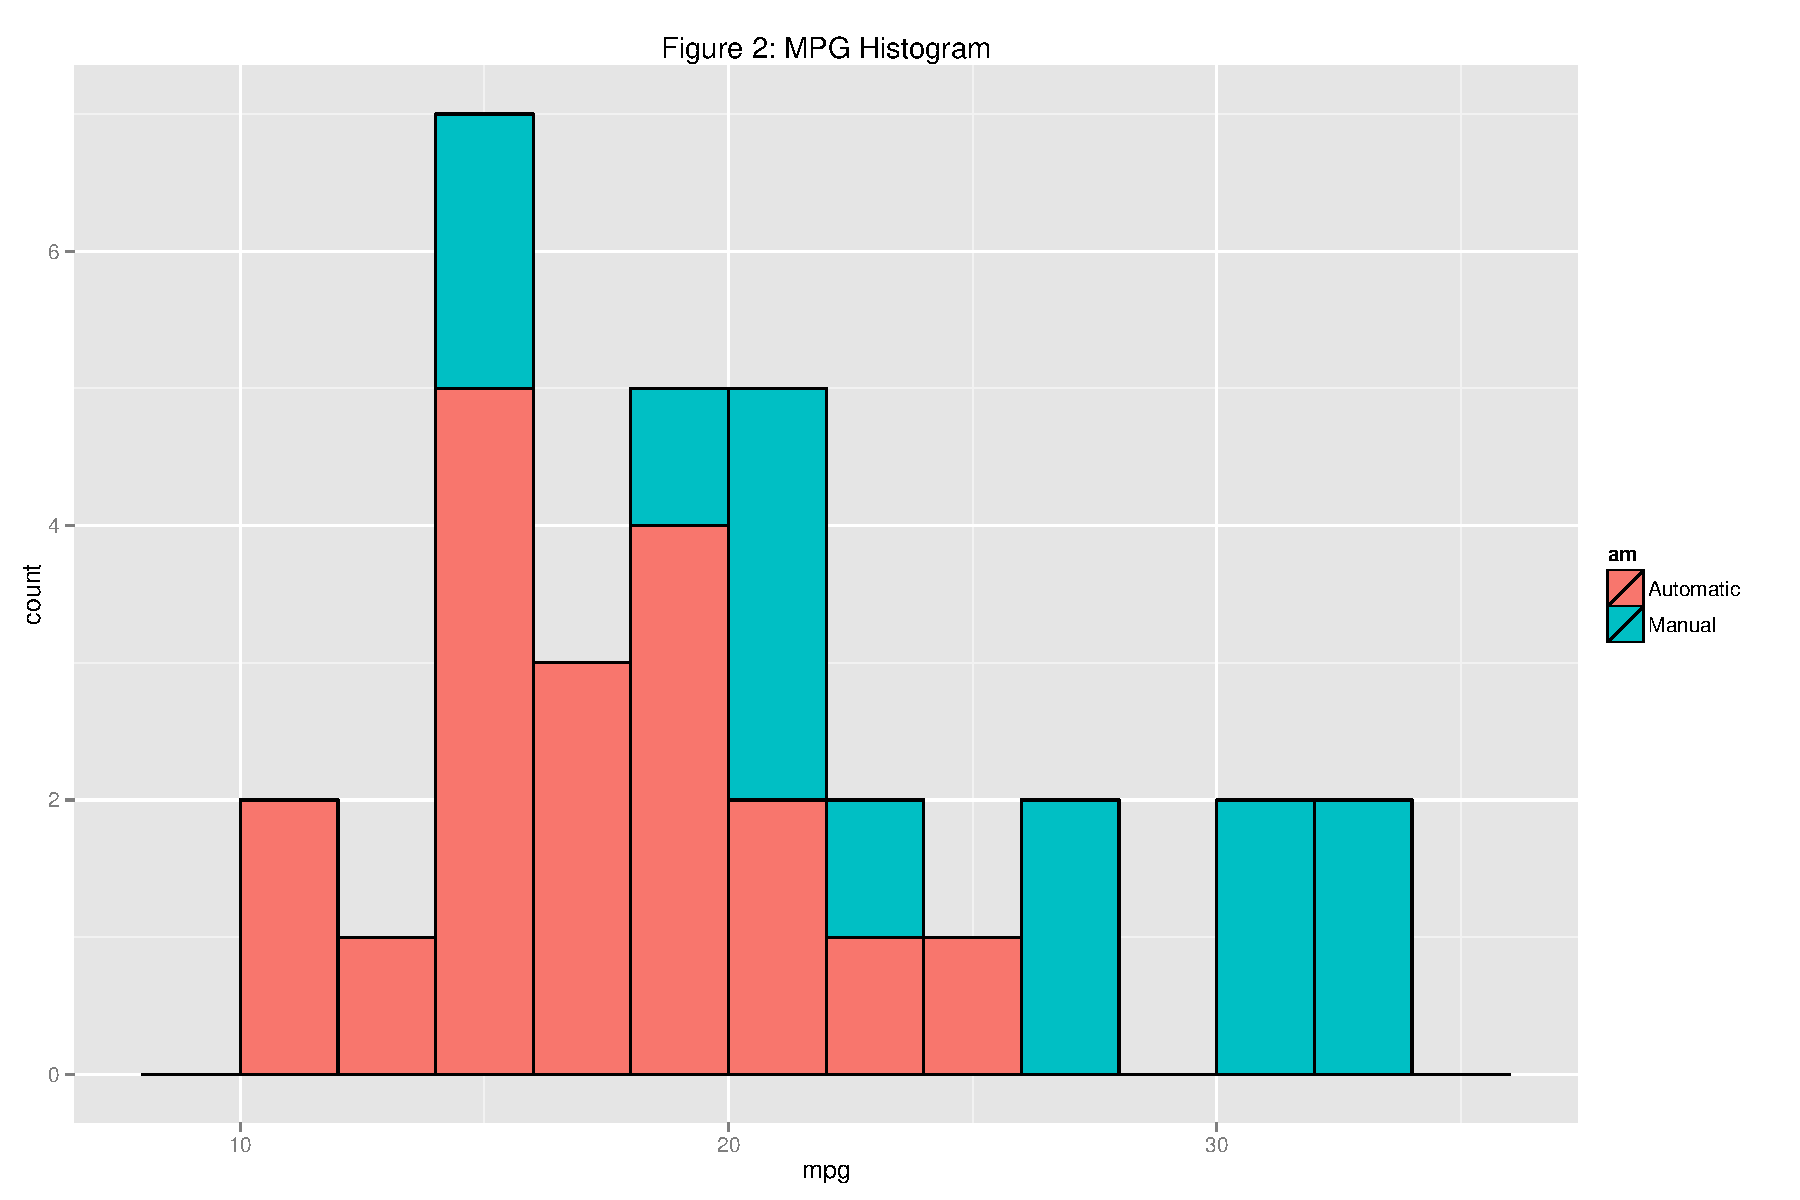
\includegraphics{figure/unnamed-chunk-11-1.pdf}

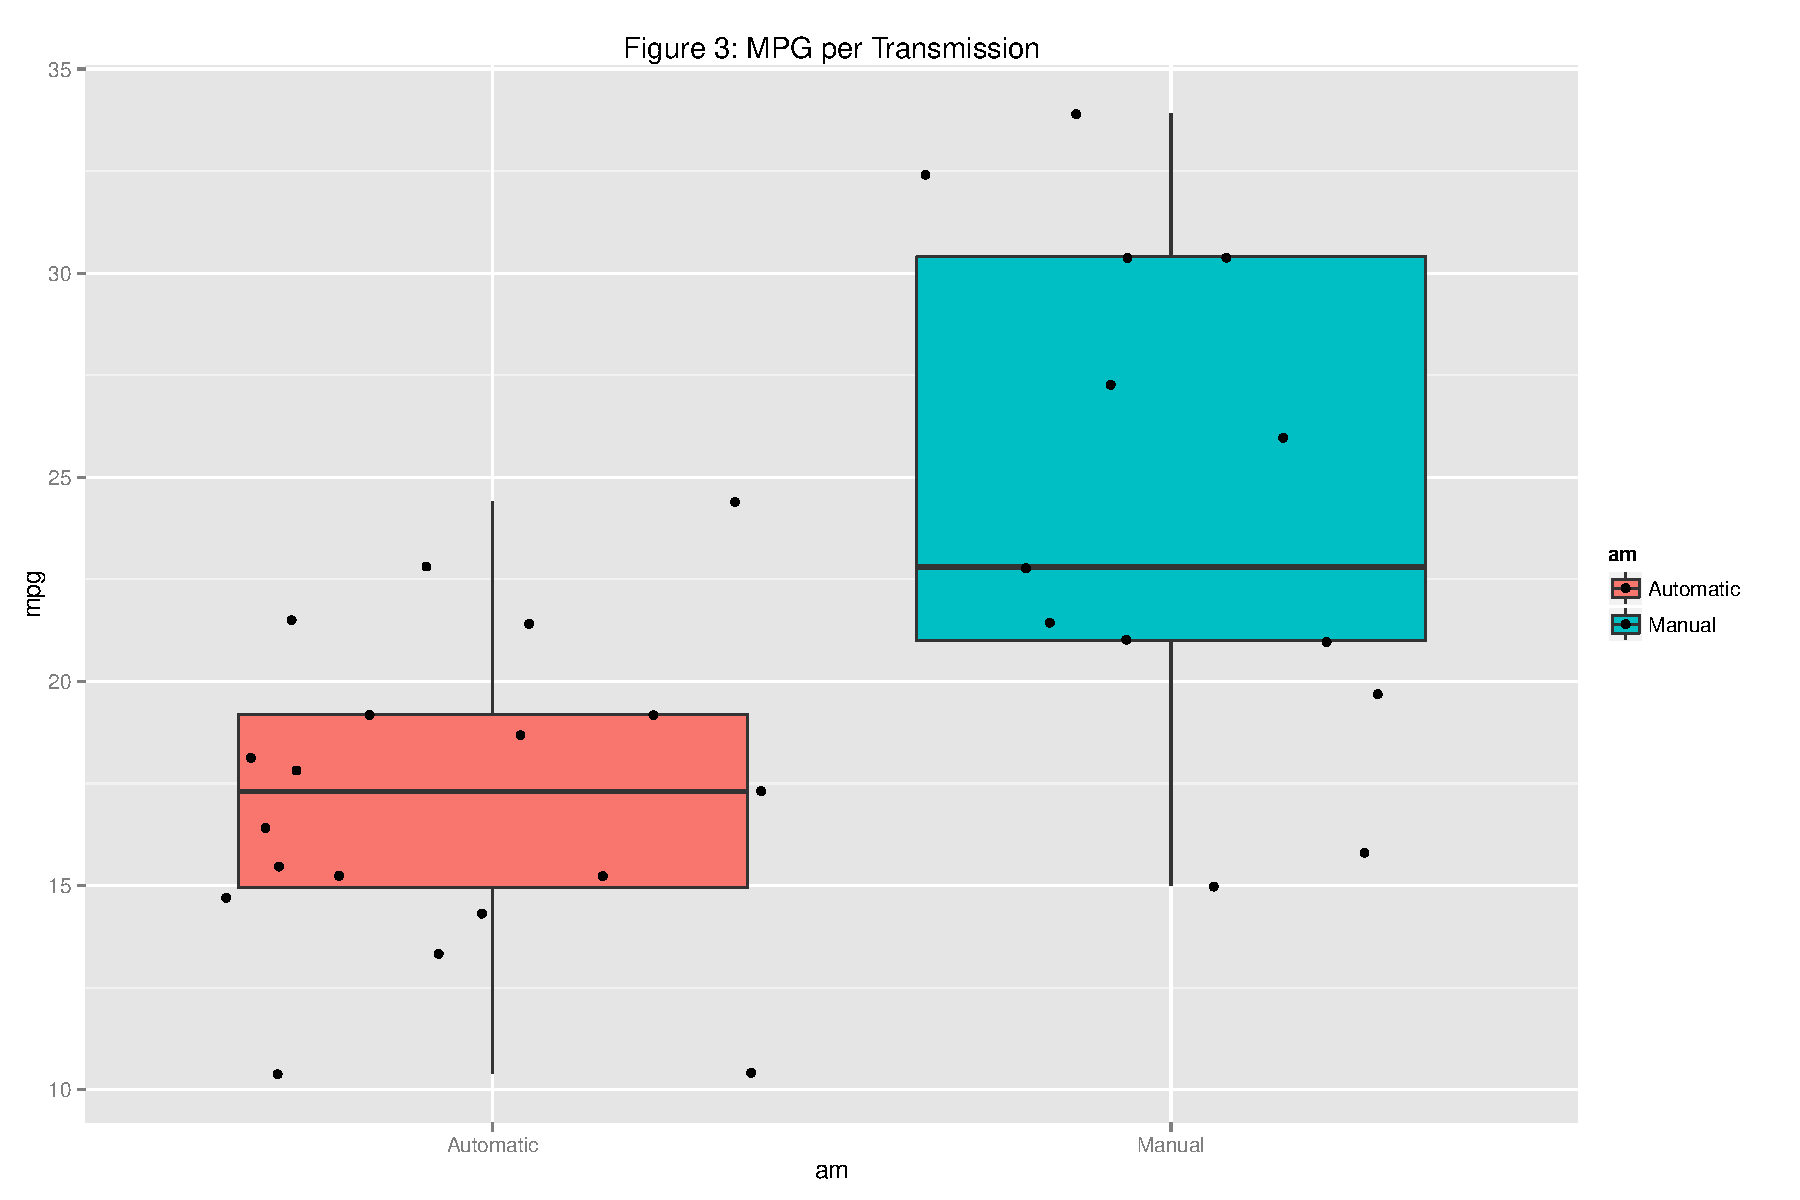
\includegraphics{figure/unnamed-chunk-12-1.pdf}

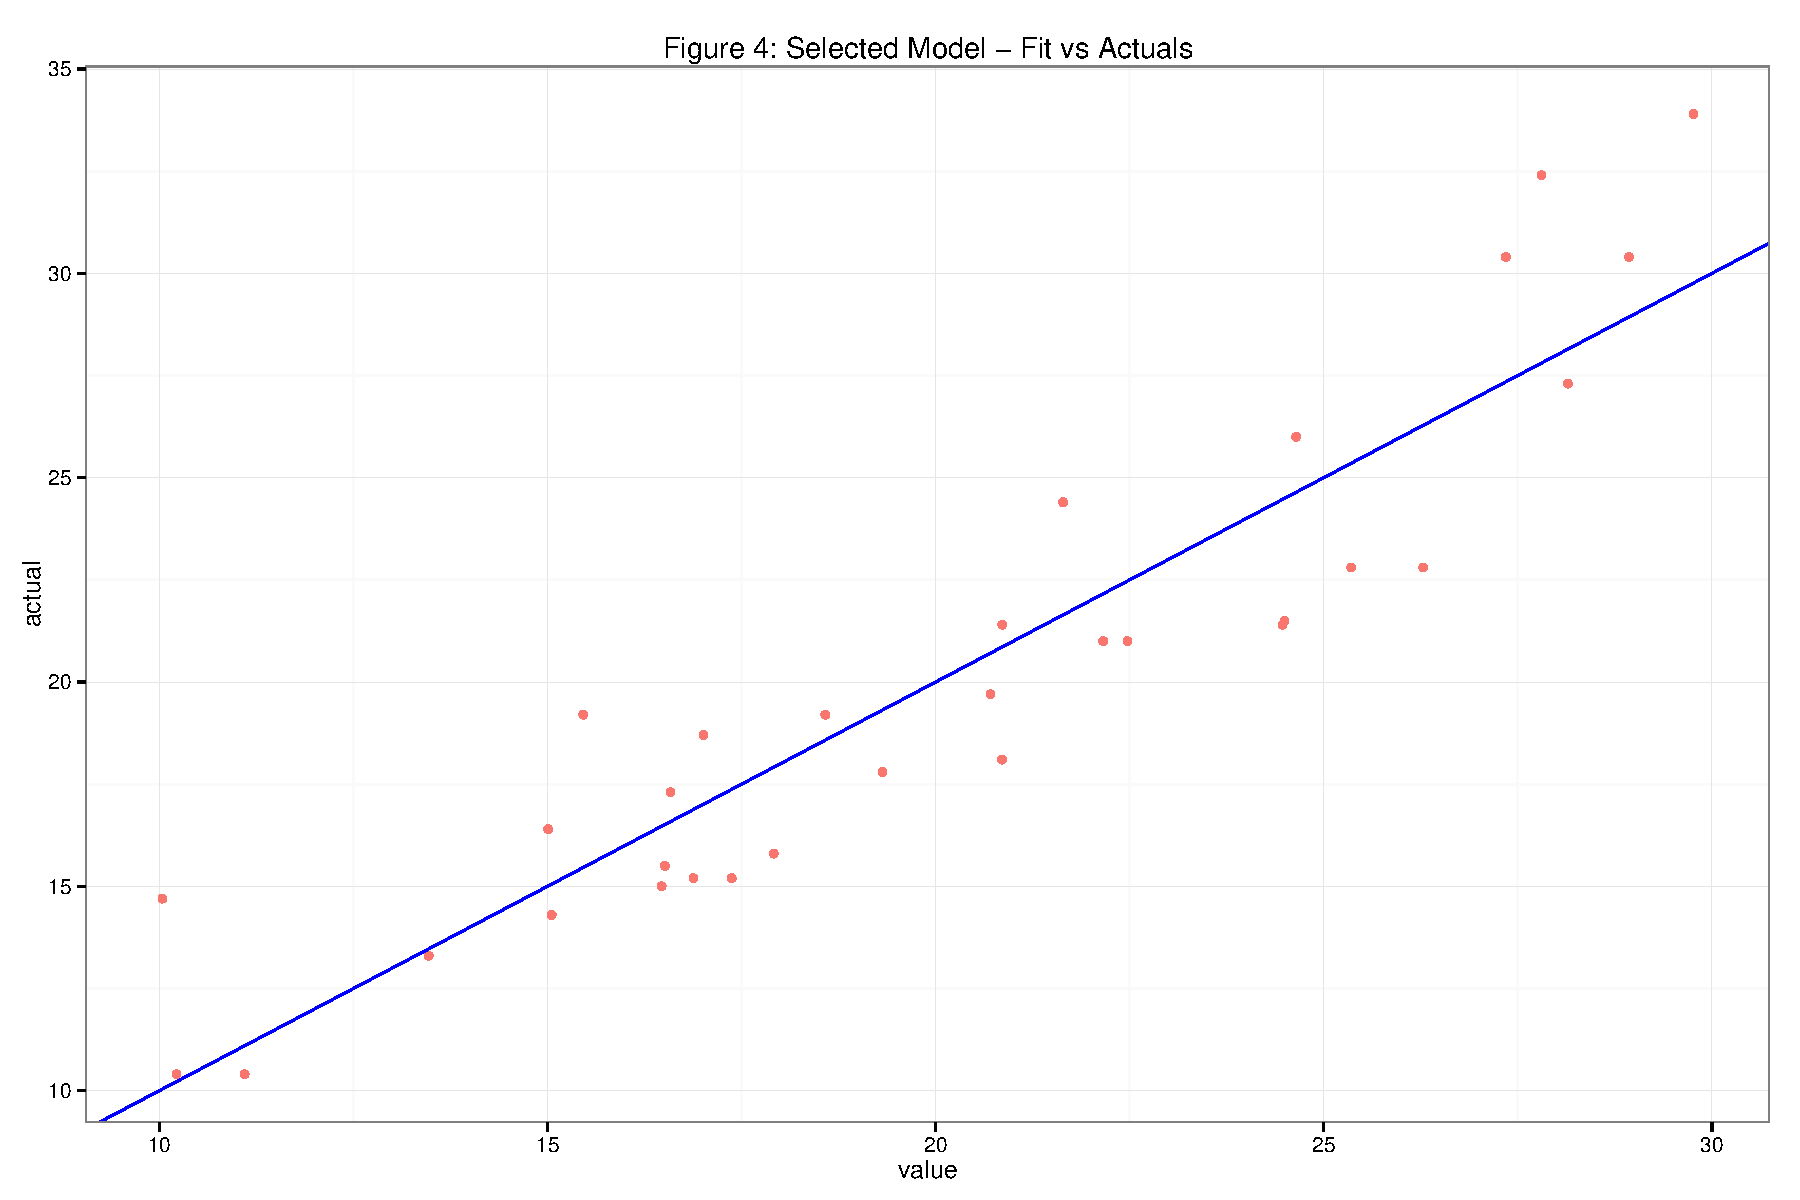
\includegraphics{figure/unnamed-chunk-13-1.pdf}

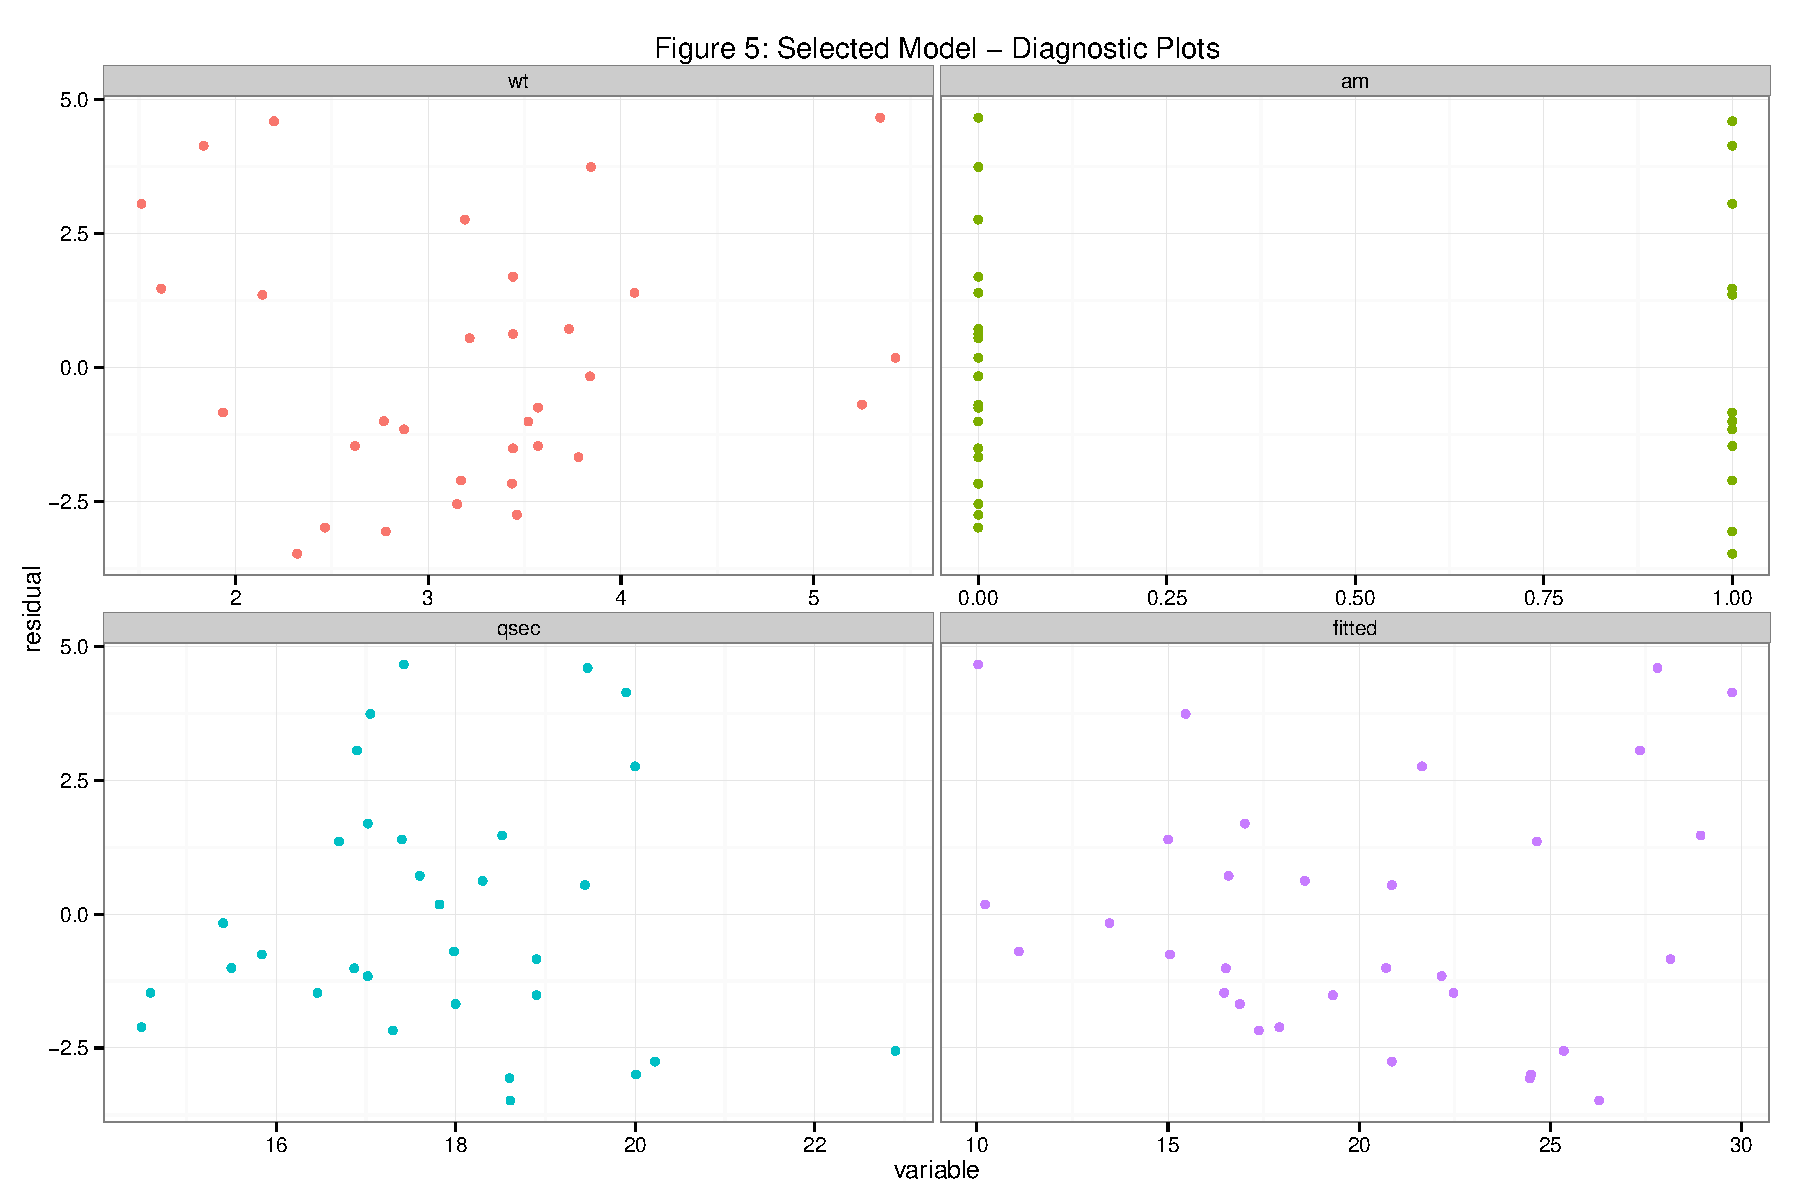
\includegraphics{figure/unnamed-chunk-14-1.pdf}

\end{document}
